\documentclass{article}
\usepackage[utf8]{inputenc}

% Paper layout
\setlength{\paperheight}{11in}
\setlength{\paperwidth}{8.5in}
\oddsidemargin 0.0in 
\evensidemargin .5in
\marginparwidth 0.07 true in
\textheight 7.5 true in
\textwidth 6.5 true in 

\PassOptionsToPackage{numbers, compress}{natbib}
\usepackage{url}
\usepackage{graphicx}
\usepackage{parskip}
\usepackage{mathtools}
\usepackage{fancyvrb}
\usepackage{array,booktabs,calc,blindtext}
% \usepackage[shortlabels]{enumerate}

%%%%%%%%%%%%%%%%%%%%%%%%%%%%%%%%%%%%%%%%%%%%%%%%%%%%%%%%%%%%%%%%%%%%%%%%%%%%%%%%

\newcommand{\hmwkTitle}{Extensible Physics Engine}
% \newcommand{\hmwkIssueDate}{22 February 2017}
\newcommand{\hmwkDueDate}{8 May 2017}
\newcommand{\hmwkClass}{6.905/6.945 Final Project Draft}
\newcommand{\hmwkClassInstructor}{Professor Gerry Sussman}
\newcommand{\hmwkAuthorName}{\textbf{Author1, Author2, Author3}}

\title{
    \textmd{\hmwkClass:\ \hmwkTitle}\\
    \\
    % \small{Issued\ on\ \hmwkIssueDate}\\
    \small{Due\ on\ \hmwkDueDate}
}
\author{\hmwkAuthorName}
\date{}
\begin{document}
\maketitle
\section{Introduction}
blah blah blah

\section{Infrastructure}
generic procedures, ps4 stuff
what we did, how we did it, why we did it

\section{Arithmetic}
vector arithmetic
what we did, how we did it, why we did it

\section{Physics Engine}
each object does its own updating, procedures are objects
what we did, how we did it, why we did it

\section{Demos}
We can easily extend our system with new forces and new objects. We begin by creating an gravity as an \texttt{interaction}:

\begin{verbatim}
(define (make-gravity thing all-things)
  (define (procedure thing influences)
    (sum (map (lambda (influence)
                (let* ((m1 (get-mass thing))
                      (m2 (get-mass influence))
                      (G 6.674e-11)
                      (v (- (get-position influence)
                                       (get-position thing)))
                      (r (magnitude v))
                      (u (/ v r))
                      (gmag (* (* G m1 m2)
                              (/ 1 (square r))))
                    )
                  (* u gmag)
                ))
              influences)))
  (let ((influences (delq thing all-things)))
    (make-interaction gravity? 'gravity procedure influences)))
\end{verbatim}

Below we've created several worlds that exhibit gravity. Once an object is added to the world, any object that has mass will feel gravitational forces with other object that have mass.

\begin{verbatim}
(define (earth-moon)
  (define w (make-world "world"))
  (define b1 (make-ball "earth" 30 1e15 #(0 0) #(0 0) "blue"))
  (define b2 (make-ball "moon" 5 1e5 #(100 100) #(-15.361 15.361) "#85929E"))
  (add-mass! b1 w)
  (add-mass! b2 w)
  w)
\end{verbatim}

\begin{verbatim}
(define (binary-stars)
  (define w (make-world "world"))
  (define b1 (make-ball "ball1" 5 1e15 #(-100 -100) #(9 -9) "red"))
  (define b2 (make-ball "ball2" 5 1e15 #(100 100) #(-9 9) "green"))
  (add-mass! b1 w)
  (add-mass! b2 w)
  w)
\end{verbatim}

\begin{verbatim}
(define (solar-system)
  (define w (make-world "world"))
  (define s (make-ball "sun" 30 1e15 #(0 0) #(0 0) "yellow"))
  (define b1 (make-ball "ball1" 5 1e5 #(100 100) #(-15.361 15.361) "blue"))
  (define b2 (make-ball "ball2" 5 1e5 #(110 110) #(-15.361 15.361) "red"))
  (define b3 (make-ball "ball3" 5 1e5 #(120 120) #(-15.361 15.361) "green"))
  (define b4 (make-ball "ball4" 5 1e5 #(130 130) #(-15.361 15.361) "purple"))
  (define b5 (make-ball "ball5" 5 1e5 #(140 140) #(-15.361 15.361) "orange"))
  (define b6 (make-ball "ball6" 5 1e5 #(150 150) #(-15.361 15.361) "gray"))

  (add-mass! s w)
  (add-mass! b1 w)
  (add-mass! b2 w)
  (add-mass! b3 w)
  (add-mass! b4 w)
  (add-mass! b5 w)
  (add-mass! b6 w)
  w
)
\end{verbatim}

\begin{figure}[h!]
  \centering
 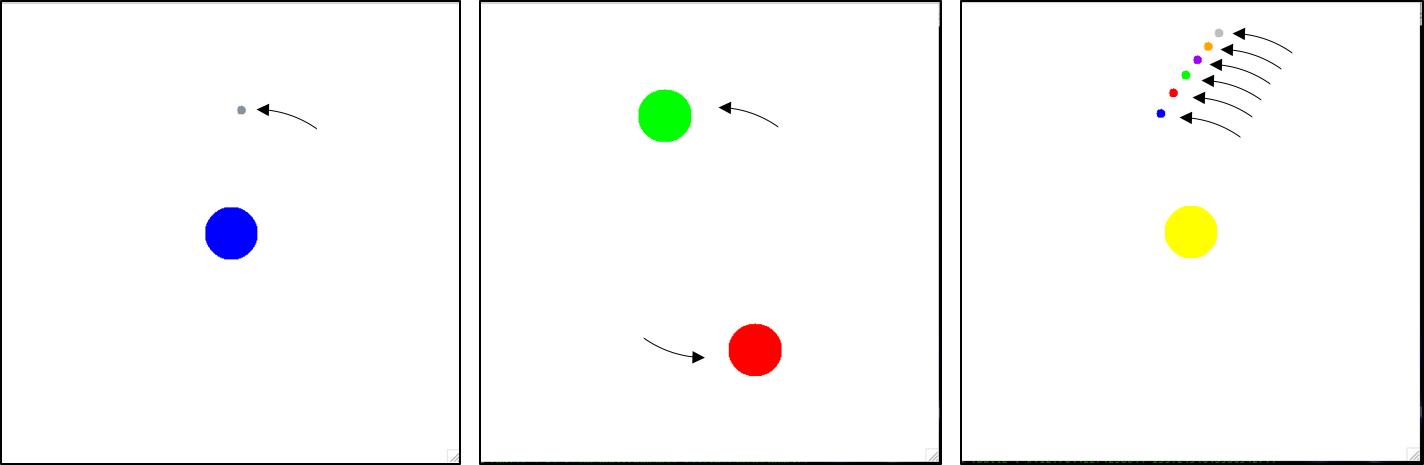
\includegraphics[width=\textwidth,height=\textheight,keepaspectratio]{figs/gravity.png}
  \caption{\textit{left}: \texttt{earth-moon}; \textit{center}: \texttt{binary-stars}; \textit{right}: \texttt{solar-system}}
  \label{figure:gravity}
\end{figure}



\begin{verbatim}
(define (magnets-1)
  (define w (make-world "world"))
  (define m1 (make-magnet "magnet1" 1e5 1 #(-30 -30) #(0 0) "red"))
  (define m2 (make-magnet "magnet2" 1e5 1 #(30 30) #(0 0) "red"))

  (add-magnet! m1 w)
  (add-magnet! m2 w)
  w
)
\end{verbatim}

\begin{verbatim}
(define (magnets-2)
  (define w (make-world "world"))
  (define m1 (make-magnet "magnet1" 5e5 1 #(-100 -100) #(0 0) "red"))
  (define m2 (make-magnet "magnet2" -5e5 1 #(100 100) #(0 0) "blue"))
  (define m3 (make-magnet "magnet3" 5e5 1 #(-100 100) #(0 0) "red"))
  (define m4 (make-magnet "magnet4" -5e5 1 #(100 -100) #(0 0) "blue"))

  (add-magnet! m1 w)
  (add-magnet! m2 w)
  (add-magnet! m3 w)
  (add-magnet! m4 w)
  w
)
\end{verbatim}

\begin{verbatim}
(define (magnetic-solar-system)
  (define w (make-world "world"))
  (define s (make-magnet "sun" 5e5 1e15 #(0 0) #(0 0) "blue"))
  (define b1 (make-magnet "ball1" -2e7 1e5 #(100 100) #(-15.361 15.361) "red"))
  (define b2 (make-magnet "ball2" -2e7 1e5 #(110 110) #(-15.361 15.361) "red"))
  (define b3 (make-magnet "ball3" -2e7 1e5 #(120 120) #(-15.361 15.361) "red"))
  (define b4 (make-magnet "ball4" -2e7 1e5 #(130 130) #(-15.361 15.361) "red"))
  (define b5 (make-magnet "ball5" -2e7 1e5 #(140 140) #(-15.361 15.361) "red"))
  (define b6 (make-magnet "ball6" -2e7 1e5 #(150 150) #(-15.361 15.361) "red"))

  (add-magnet! s w)
  (add-magnet! b1 w)
  (add-magnet! b2 w)
  (add-magnet! b3 w)
  (add-magnet! b4 w)
  (add-magnet! b5 w)
  (add-magnet! b6 w)
  w
)
\end{verbatim}



\end{document}





